\chapter{Execution and Results}\label{ch:execandresults}

Our research consisted of four networks: ACGAN, DCGAN, InfoGAN and WGAN. Each of the networks was trained for 20,000 epochs each. The training period for the individual networks took anywhere between a few hours and a couple of days. For each network, we logged a few key metrics, mainly the Generator Loss (GLoss), Discriminator Loss (DLoss) and the Accuracy (Acc). 
\par\bigskip
Below we show graphically the performance of the (four) classical networks as compared to the CapsNet discriminator augmented networks.

\begin{figure}[H]
    \centering
    \subfloat[Classical ACGAN]{{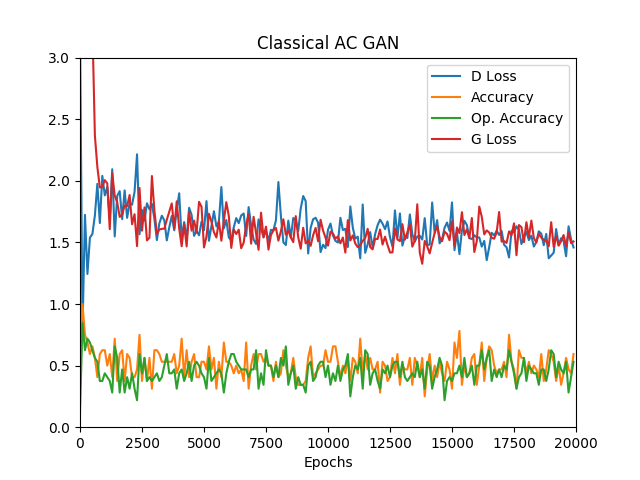
\includegraphics[width=.45\linewidth]{images/plots/classacgan.png} }}%
    \qquad
    \subfloat[CapsNet augmented ACGAN]{{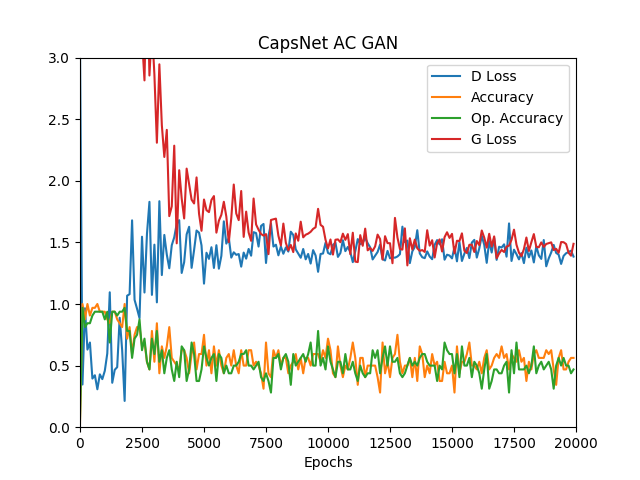
\includegraphics[width=.45\linewidth]{images/plots/capsacgan.png} }}%
    \caption{ACGAN metrics}%
    \label{fig:acgan}%
\end{figure}

\begin{figure}[H]
    \centering
    \subfloat[Classical DCGAN]{{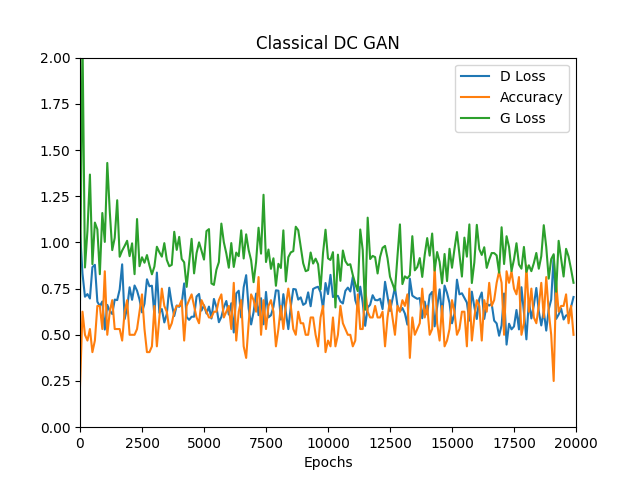
\includegraphics[width=.45\linewidth]{images/plots/classdcgan.png} }}%
    \qquad
    \subfloat[CapsNet augmented DCGAN]{{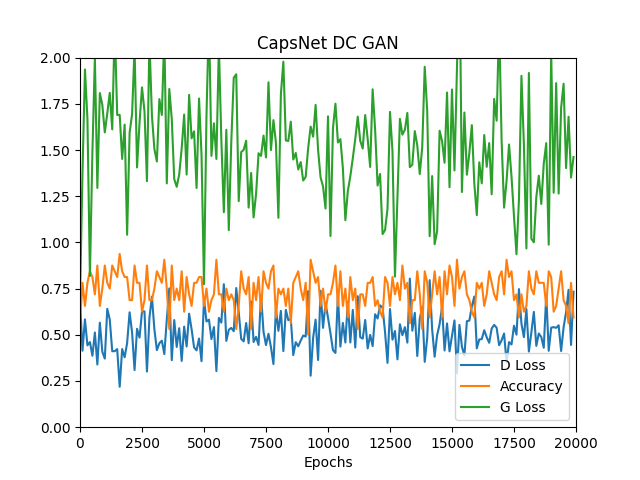
\includegraphics[width=.45\linewidth]{images/plots/capsdcgan.png} }}%
    \caption{DCGAN metrics}%
    \label{fig:dcgan}%
\end{figure}

\begin{figure}[H]
    \centering
    \subfloat[Classical InfoGAN]{{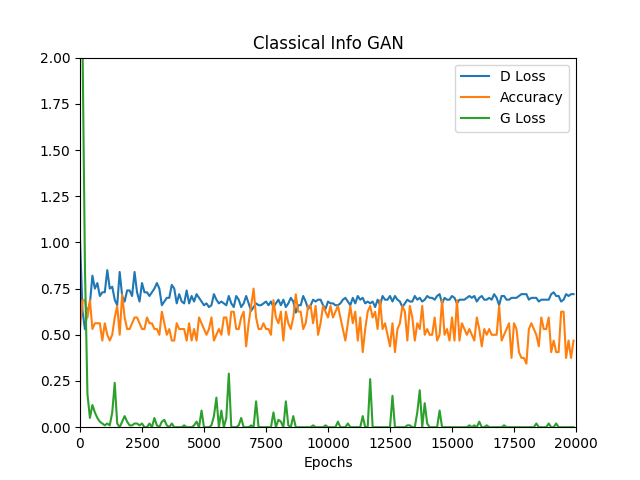
\includegraphics[width=.45\linewidth]{images/plots/classinfogan.png} }}%
    \qquad
    \subfloat[CapsNet augmented InfoGAN]{{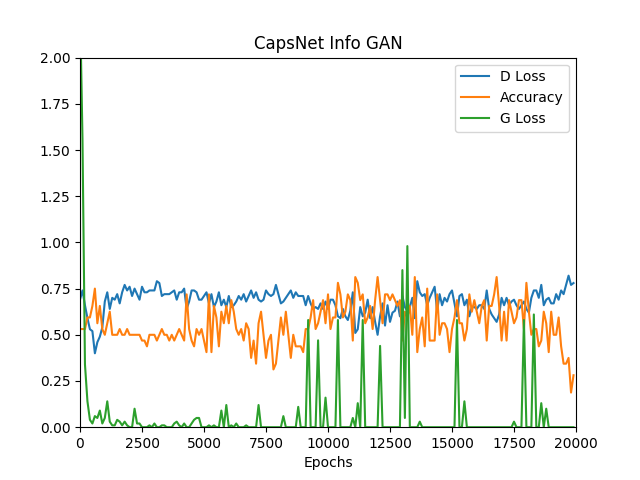
\includegraphics[width=.45\linewidth]{images/plots/capsinfogan.png} }}%
    \caption{InfoGAN metrics}%
    \label{fig:infogan}%
\end{figure}

\begin{figure}[H]
    \centering
    \subfloat[Classical WGAN]{{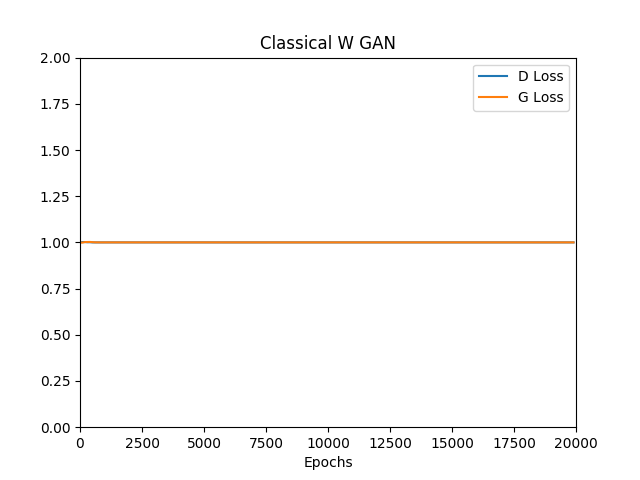
\includegraphics[width=.45\linewidth]{images/plots/classwgan.png} }}%
    \qquad
    \subfloat[CapsNet augmented WGAN]{{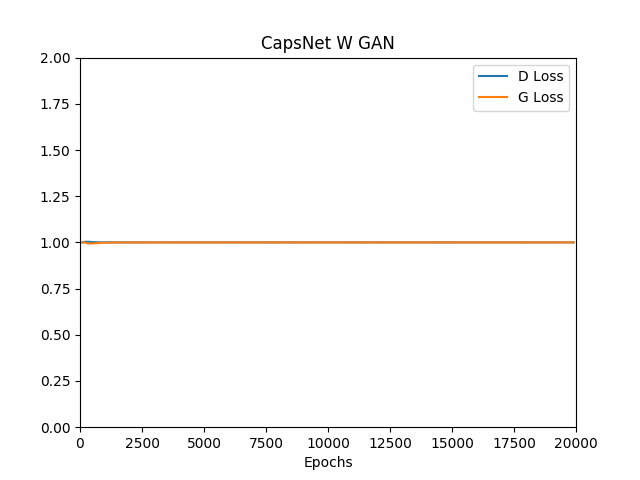
\includegraphics[width=.45\linewidth]{images/plots/capswgan.png} }}%
    \caption{WGAN metrics}%
    \label{fig:wgan}%
\end{figure}

The metrics of WGAN are at a smaller scale, so below is a comparison at the lower scale.

\begin{figure}[H]
    \centering
    \subfloat[Classical WGAN]{{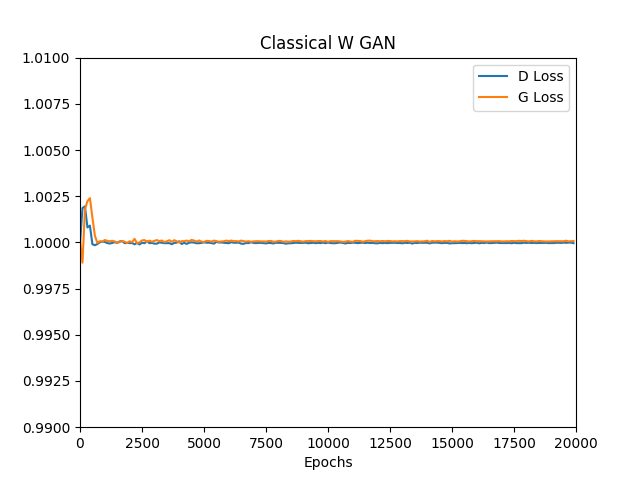
\includegraphics[width=.45\linewidth]{images/plots/classwgan-zoomed.png} }}%
    \qquad
    \subfloat[CapsNet augmented WGAN]{{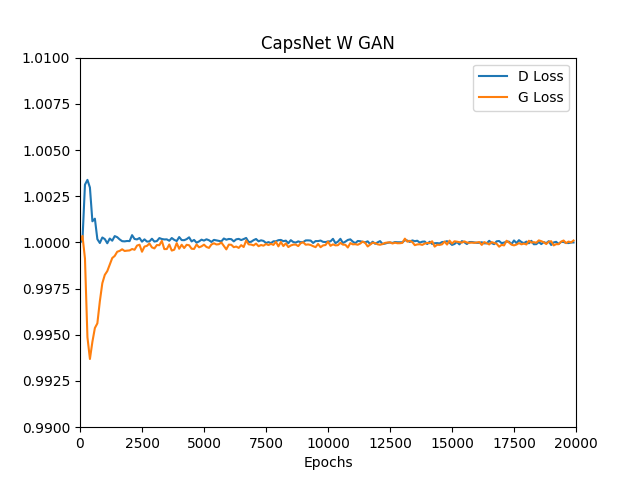
\includegraphics[width=.45\linewidth]{images/plots/capswgan-zoomed.png} }}%
    \caption{WGAN metrics - zoomed}%
    \label{fig:wgan}%
\end{figure}
\par\bigskip

A preliminarily analysis of the data shows us that our CapsNet augmented networks, hence-forth referred to as the network name prefixed with "Caps", perform comparably with the classical architectures. 
\par\bigskip

Under ACGAN we see that CapsACGAN starts off with very high variance in GLoss and DLoss. Over the course of 20,000 epochs, the variance gradually reduces to match the Classical ACGAN metrics at the end. Accuracy of CapsACGAN, on the other hand, quickly stabilizes to meet classical ACGAN metrics. As a side note, ACGAN was the fastest trained network, taking roughly three hours to complete 20,000 epochs.
\par\bigskip

DCGAN and InfoGAN are interesting in the sense that they show a remarkable shift in the GLoss metric. This is odd considering only the discriminator code was augmented and the generator was left untouched. This requires further analysis. Accuracy and DLoss follow their classical counterpart closely.
\par\bigskip

WGAN happens to be the best and state-of-the-art. Consequently, the variance in the metrics were at a much smaller scale. We had to zoom-in to notice the difference between the metrics. We see that an initial burst of high variance quickly stabilizes to quickly trace a path closely matching the classical architecture.
\par\bigskip

